

\chapter{Results}
\label{cha:results}

% Move this to Ericssons appendix
%\section{Positive feedback on fan and overheating faults}
%\noindent\fbox{
%	\parbox{\textwidth}
%	{
%		Comment on the fan issue found while mining faults
%	}
%}


\section{Comparative imputing experiments}
\label{sec:imp-exps}

A set of thorough experiments has been designed to compare both model estimation techniques and empirically determine which one performs better for the current dataset.

The starting point is a database containing approximately two months of measurements from several \acp{rbs}. Then, the database is mined to find $n=50$ signals per feature with no missing data. After that, data has been artificially removed at a set ratio using a uniform distribution so that it can be simulated a \ac{mcar} scenario \cite{rantou2017missing}. 

The two algorithms run to estimate the process models and use them to run the Kalman smoothing. It is used the coefficient of determination $R^2$ to compare the performance of the models. 

\begin{equation}\label{eq:R2}
	R^2 = 1 - \frac{\sum_{i}{(y_i - \hat{y}_i)^2}}{\sum_{i}{(y_i - \bar{y})^2}}
\end{equation}

Where $y_i$ refers to the $i$-th data sample, $\hat{y}$ its estimated value and $\bar{y}$ the series mean. 

Thus, having perfect predictions would cancel out the right-hand term's numerator and produce a score equal to 1. Therefore, the closer the score is to 1, the better quality has been the data imputation.  

The process of removing data, imputing and computing the coefficient of determination value is performed iteratively while increasing the amount of simulated missing data. The mean of the $R^2$ values from the  selected \ac{rbs} are reported. 

In Figure \ref{alg:imputing_exp}, it is shown the experiment's algorithm pseudocode in order to give more context of the meaning of the results plots.

\begin{figure}[hptb]
\begin{lstlisting}[keywords={,let, input, output, return, datatype, function, in, if, else, foreach, while, begin, end, do, }, mathescape=true, tabsize=4, basicstyle=\ttfamily\small]
input : database, ratio_step, ratio_min, ratio_max
output: mean_scores

let n $\gets$ rbs batch size
let grid $\gets$ [ratio_min : ratio_step : ratio_max]
let mean_scores $\gets$ []

foreach feature in database.get_features() do:
	sites $\gets$ database.get_random_sites(n)
	i $\gets$ 0
	foreach ratio in grid do:
		let arima_scores $\gets$ []
		let structural_scores $\gets$ []
		j $\gets$ 0
		foreach site in sites do:
			data $\gets$ database.get_site_data(site, feature)
			sim_data $\gets$ remove_uniform_random_data(data, ratio)
			
			imputed_arima $\gets$ impute_with_arima(sim_data)
			imputed_structural $\gets$ impute_with_structural_model(sim_data)
			
			arima_scores[j] $\gets$ $R^2$(data, imputed_arima)
			structural_scores[j] $\gets$ $R^2$(data, imputed_structural)
			j $\gets$ j + 1
		mean_scores[i] $\gets$ (ratio, mean(arima_scores), mean(structural_scores))
		i $\gets$ i + 1
return mean_scores
\end{lstlisting}
\caption{Comparative imputing experiment pseudocode.}
\label{alg:imputing_exp}
\end{figure}

\pagebreak

Figure \ref{fig:imp_exp_good} shows the results of the imputation comparison for the radio traffic as example. It can be seen that the $R^2$ value decreases --as expected-- when the missing data ratio increase. It also can be seen that, in this example, and most of them, structural models performs better than ARIMA models for imputing.

\begin{figure}[hptb]
	\centering
	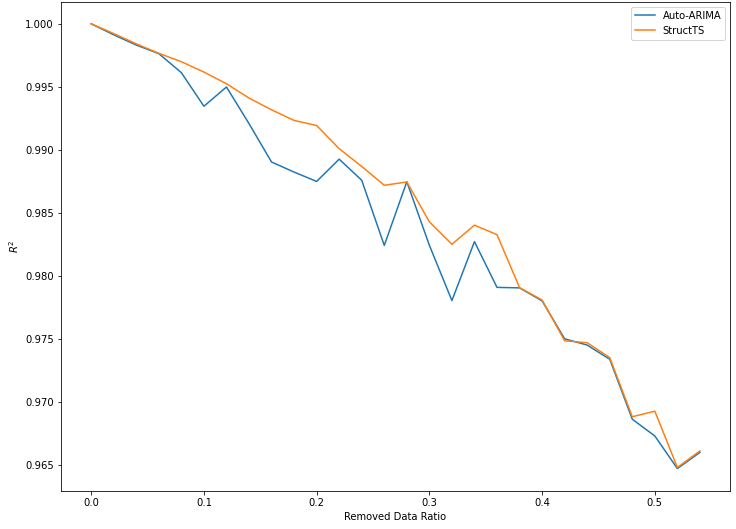
\includegraphics[width=0.7\textwidth]{imp_traffic}
	\caption{Radio traffic load imputation}
	\label{fig:imp_exp_good}
\end{figure}

%\begin{figure}[hptb]
%	\centering
%	\begin{subfigure}{.48\textwidth}
%		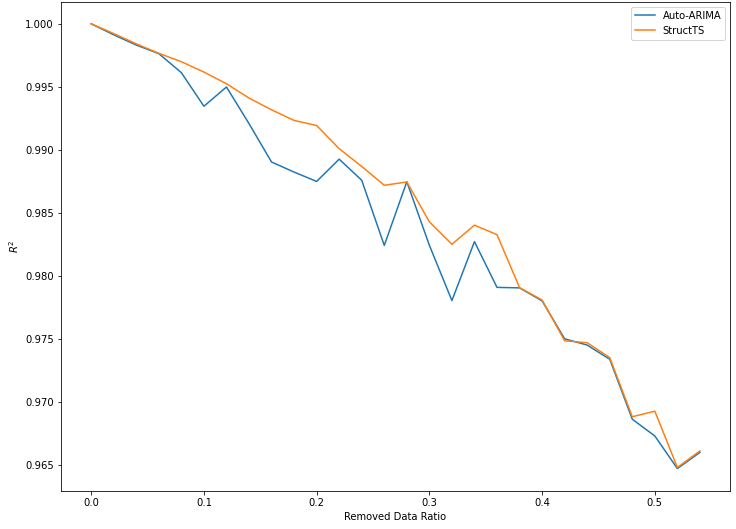
\includegraphics[width=\textwidth]{imp_traffic}
%		\caption{Radio traffic load imputation}
%		\label{fig:imp_radio_traffic}
%	\end{subfigure}%
%	\hfill
%	\begin{subfigure}{.48\textwidth}
%		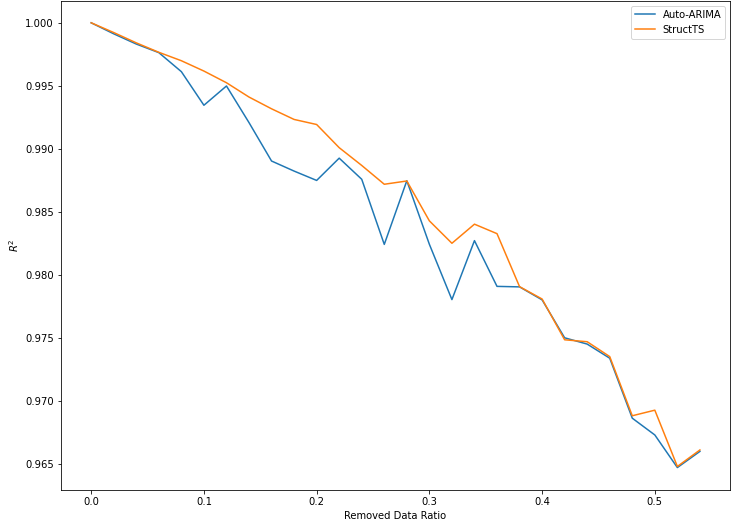
\includegraphics[width=\textwidth]{imp_temp}
%		\caption{Cabinet temperature imputation}
%		\label{fig:imp_temp}
%	\end{subfigure}
%	\caption{Imputation experiments good results}
%	\label{fig:imp_exp_good}
%\end{figure}


Although promising results were obtained for some of the imputed signals, there were other cases where the experiment did not perform as expected. In the following subsections, they will be discussed.

\subsection{Unintuitive $R^2$ values}

There are cases in which Auto-ARIMA estimation show poor and even negative $R^2$ values as shown in Figure \ref{fig:imp_exp_issue}. These are unintuitive results, as $R^2$ values are usually expected to be limited to the $[0,1]$ interval. 

Nonetheless, this is meant only for linear models, where the worst fitted model is assumed to be the observations mean \cite{wackerly}. Thus, having negative $R^2$ values implies that the observations mean explains more variance than the fitted model.

\begin{figure}[hptb]
	\centering
	\begin{subfigure}{.48\textwidth}
		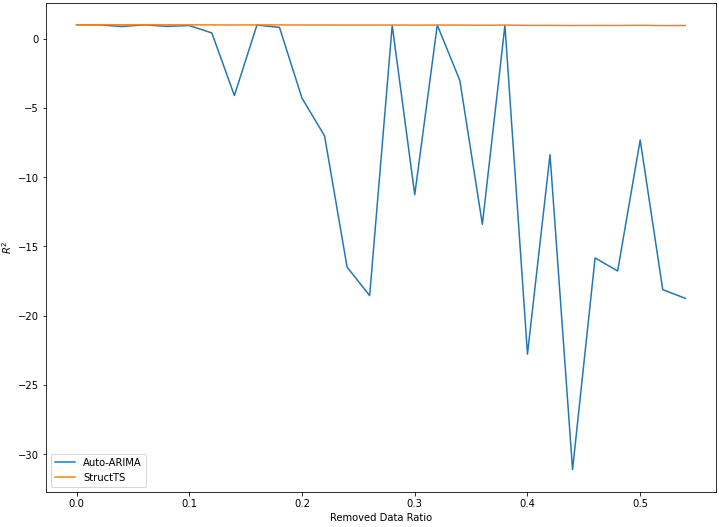
\includegraphics[width=\textwidth]{imp_sys_voltage}
		\caption{\ac{pdu} system voltage imputation.}
		\label{fig:imp_pdu_sys_voltage}
	\end{subfigure}%
	\hfill
	\begin{subfigure}{.48\textwidth}
		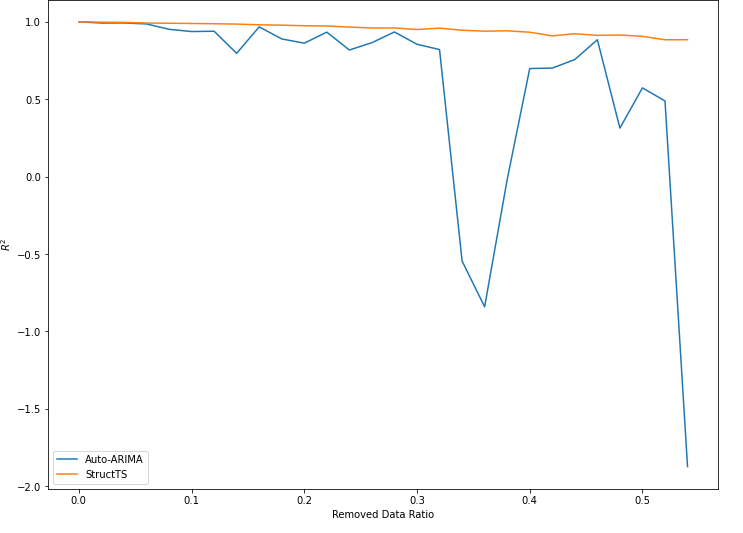
\includegraphics[width=\textwidth]{imp_power_load}
		\caption{Average \ac{psu} utilisation imputation.}
		\label{fig:imp_psu_load}
	\end{subfigure}
	\caption{Imputation experiments with bad results.}
	\label{fig:imp_exp_issue}
\end{figure}

\subsection{Optim convergence failures}

The model estimation threw runtime exceptions for some features due to the R code calls to the \texttt{optim} library not converging. These exceptions were found to be an actual bug in the library that occurs when the function being optimised tends to a constant value as shown in Figure \ref{fig:imp_conv_issue}. A dedicated routine was written to catch whenever this exception was thrown and run a simple interpolation instead of estimating the model.

\begin{figure}[H]
	\centering
	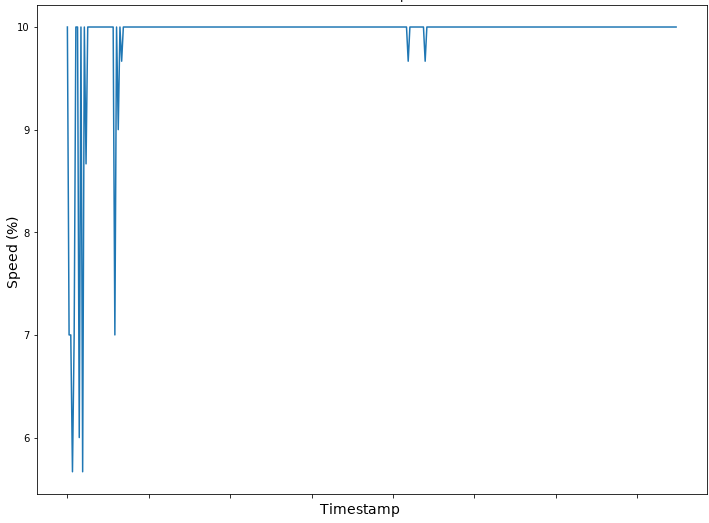
\includegraphics[width=0.55\linewidth]{imp_conv_issue}
	\caption{Example of problematic signals for Auto-ARIMA estimation.}
	\label{fig:imp_conv_issue}
\end{figure}

\subsection{Conclusion of the imputing experiments}

The imputations using ARIMA models have shown to be unstable for some signals. Even though when, for the same signals, the structural model does not overperform either, it stills better than the very negative $R^2$ scores produced by the ARIMA approximations. In conclusion, based on this experiment's results, the structural models' approach has been chosen to impute the missing data and construct the database. 


\section{Forecasting initial experiments}


The average \ac{psu} load signal shown in Figure \ref{fig:forecast_experiment_signal} has been chosen to run the following experiments. It is not a particularly easy signal since it contains some severe outliers in the first days that turned the power to almost zero, and in the end, the average power consumption seems to decrease.

It is necessary to notice that in every forecasting model, the further the prediction horizon is, the more uncertainty and, thus, the lower performance. For this experiment, it has been decided to leave the last 10\% of data for testing purposes.

\begin{figure}[H]
	\centering
	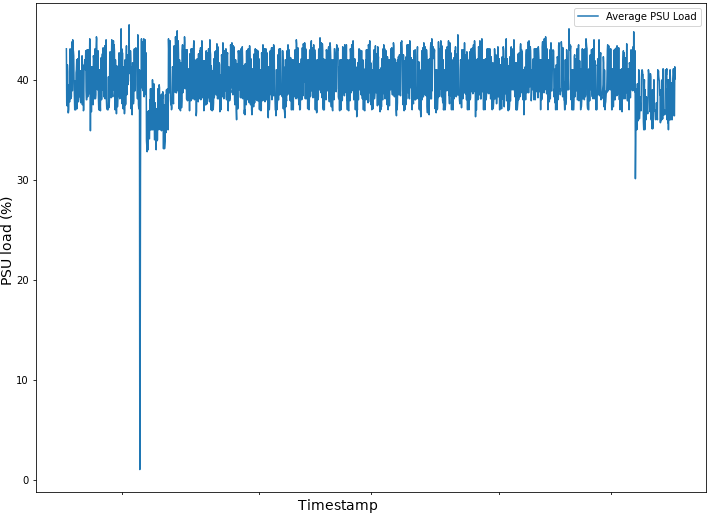
\includegraphics[width=0.6\linewidth]{forecast_experiment_signal}
	\caption{Average PSU load signal used for the forecasting experiments}
	\label{fig:forecast_experiment_signal}
\end{figure}

In the following sections, the baselines models will be implemented first. Then, results of the univariate Prophet model will be shown. %To, later, add more exogenous regressors to observe how the predictions are improved. 
The models will be evaluated by using the scores described in Section \ref{subsec:eval_criteria}.

\subsection{Evaluation criteria}\label{subsec:eval_criteria}
\subsubsection*{Coefficient of determination}

As previously mentioned, the coefficient of determination $R^2$ is a measure of how much variance of $\hat{y}$ is explained by the variance in $y$ in a linear regression context. It is compared against the considered \emph{worst possible linear approximation} which corresponds to the samples mean.

Although the current application is not linear, $R^2$ is still considered a valuable score to compare predictor performances. Nonetheless, as the linearity assumption is not met, its values would reside in $(-\infty, 1]$, where 0 still is the mean value, but it is no longer considered the worst possible fit.

%\begin{equation}\label{eq:rsq}
%	R^2 = 1 - \frac{\sum_{i}{(y_i - \hat{y}_i)^2}}{\sum_{i}{(y_i - \bar{y}_i)^2}}
%\end{equation}


\subsubsection*{Mean absolute error}

It measures, in absolute terms, the deviations from the true values. \ac{mae} is preferred, given its interpretability, over \ac{rmse} \cite{MAE}.

\begin{equation}\label{eq:mae}
	\text{MAE}	= \frac{1}{N} \sum_{i=1}^{N}{ \left| y_i - \hat{y}_i \right| }
\end{equation}


\subsubsection*{Mean out-of-bounds error}

As a result of the fitting or forecasting process, Prophet's output is comprised by the mean prediction $\hat{y}_t$ and also its lower and upper boundaries $\hat{y}_t - \Delta\hat{y}_t$ and $\hat{y}_t + \Delta\hat{y}_t$, respectively. Where $\Delta \hat{y}_t$ is the computed confidence interval half-magnitude for the time $t$. The width of this interval is defined by the user and defaults to $80\%$ 

Let  the \ac{obe} be the out-of-confidence-bands error defined as zero if the true value $y_t$ lies inside the confidence interval, and if it lies outside, define the distance to the closest confidence boundary as defined in (\ref{eq:obe}). Then the \ac{mobe} of $N$ samples can be obtained by taking the mean of these values to obtain an overall performance score as in (\ref{eq:mobe}). 

\begin{equation}
	\text{OBE}_t = 
	\begin{cases}
		\hfil 0  & \text{, if } \hat{y}_t - \Delta\hat{y}_t \leq y_t \leq \hat{y}_t + \Delta\hat{y}_t \\
		\bm{\min} \Big\{ \big| y_t - (\hat{y}_t - \Delta\hat{y}_t) \big| , \big	| y_t - (\hat{y}_t + \Delta\hat{y}_t) \big| \Big\} & \text{, otherwise}\\
	\end{cases}\label{eq:obe} 
\end{equation}
	
\begin{equation}
	\label{eq:mobe}
	\text{MOBE} = \frac{1}{N} \sum_{t=1}^{N}{ \text{OBE}_t }
\end{equation}

\subsection{Baseline predictions models}

For the imputation step, the seasonal ARIMA and structural models have been learnt to fill the missing values by applying the Kalman smoothing algorithm. Furthermore, these models can also be used to forecast future observations. They are not expected to overperform. Nonetheless, predicting with them can be used as a benchmark to compare other models' improvements over their baseline.  

\subsubsection*{Structural model predictions}
\label{subsubsec:structts_preds}

Figure \ref{fig:base_sts_overall} shows the overall performance of the structural time series predictor. It can be seen that its predictive mean tends to follow the test dataset mean, whereas the confidence interval is wider the further the prediction horizon is. More detailed plots are available in Appendix \ref{app:structts_preds}.

\begin{figure}[H]
	\centering
	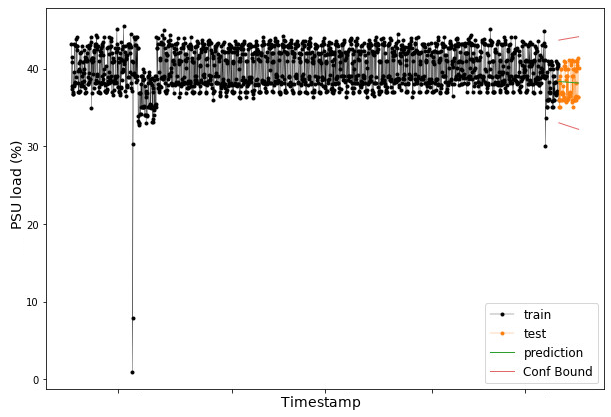
\includegraphics[width=0.8\linewidth]{baseline_imp_overall-sts}
	\caption{Structural model 3-days baseline overall performance}
	\label{fig:base_sts_overall}
\end{figure}

When plotting how the predictions $\hat{y}$ and the real values $y$ are distributed, the ideal prediction would be denoted by the positive unitary line. Therefore, the results in Figure \ref{fig:base_sts_joints} can be considered very poor.

\begin{figure}[H]
	\centering
	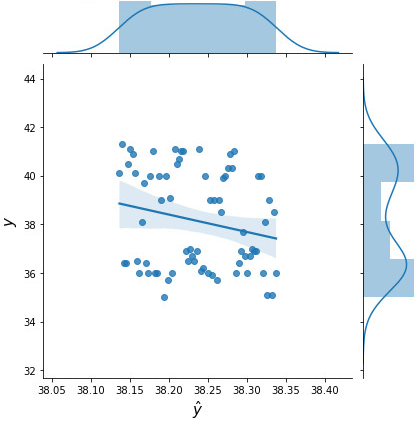
\includegraphics[width=0.55\linewidth]{baseline_imp_joints-sts}
	\caption{Structural model 3-days baseline joint distribution}
	\label{fig:base_sts_joints}
\end{figure}


\subsubsection*{Auto-ARIMA implementation}

Same as in Section \ref{subsubsec:structts_preds}, an Auto-ARIMA model is trained and used to make predictions. In this case, it can be seen that, in the short-range, the predictive mean tries, but poorly succeeds to follow the actual data fluctuations. However later, in the long-range, it converges to the data mean. More detailed plots of the results can be found in Appendix \ref{app:arima_preds}.   

\begin{figure}[H]
	\centering
	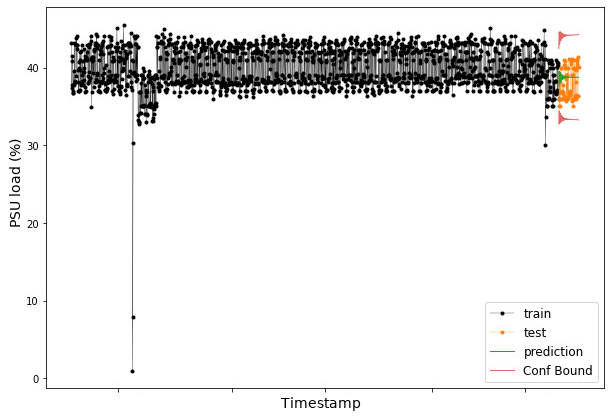
\includegraphics[width=0.8\linewidth]{baseline_imp_overall}
	\caption{Auto-ARIMA 3-days baseline overall performance}
	\label{fig:base_arima_overall}
\end{figure}

Although the joint distribution of predictions and true values has been slightly improved, it still is very poor.

\begin{figure}[H]
	\centering
	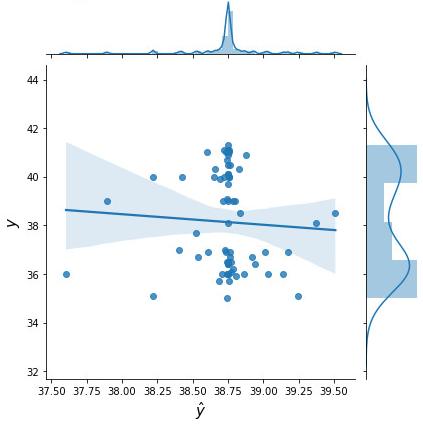
\includegraphics[width=0.55\linewidth]{baseline_imp_joints}
	\caption{Auto-ARIMA 3-days baseline joint distribution}
	\label{fig:base_arima_joints}
\end{figure}

\subsubsection*{Overall baselines scores}

In Table \ref{table:base_scores}, the long-range prediction of both baselines is summarised. They perform very poorly; nonetheless, as naive baselines, it is not expected any other outcome.

\begin{table}[H]
	\centering
	\begin{tabular}{|c|c|c|}
		\hline
		Score		& Structural Model	& Auto-ARIMA \\
		\hline
		\ac{mae} 	&  1.87 			& 1.95 \\
		$R^2$ 		& -0.02				& -0.12 \\
		\ac{mobe} 	&  0				& 0 \\
		\ac{rmse}	& 2.02 				& 2.12 \\
		\hline
	\end{tabular}
	\caption{Baselines long-range performance}
	\label{table:base_scores}
\end{table}

\subsection{Univariate Prophet model implementation}

Figure \ref{fig:prophet_uni_split} shows the complete results of training and testing for a univariate Prophet model. In comparison to the baselines, now it can be observed that the predictive mean tends to follow a more clear seasonal pattern. Nonetheless, in the testing set, it appears to miss the trend change.

\begin{figure}[H]
	\centering
	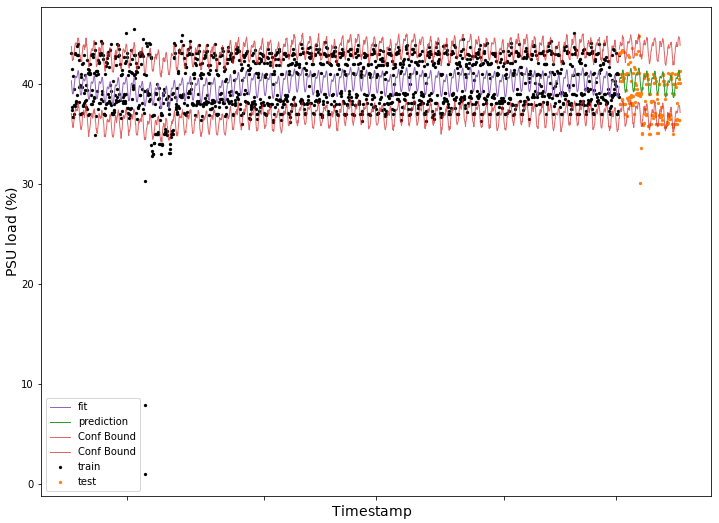
\includegraphics[width=0.8\linewidth]{prophet_uni_split}
	\caption{Training, test and predictions from the univariate Prophet model}
	\label{fig:prophet_uni_split}
\end{figure}

More detailed plots can be found in Appendix \ref{app:uniprophet}.


\subsubsection*{Model learnt components}

Figure \ref{fig:prophet_uni_components} presents the learnt approximation of every component in the \ac{gam}. Although the trend did not overfit the outliers, it stills learnt that there is a breakpoint and changed the piecewise trend.

\begin{figure}[H]
	\centering
	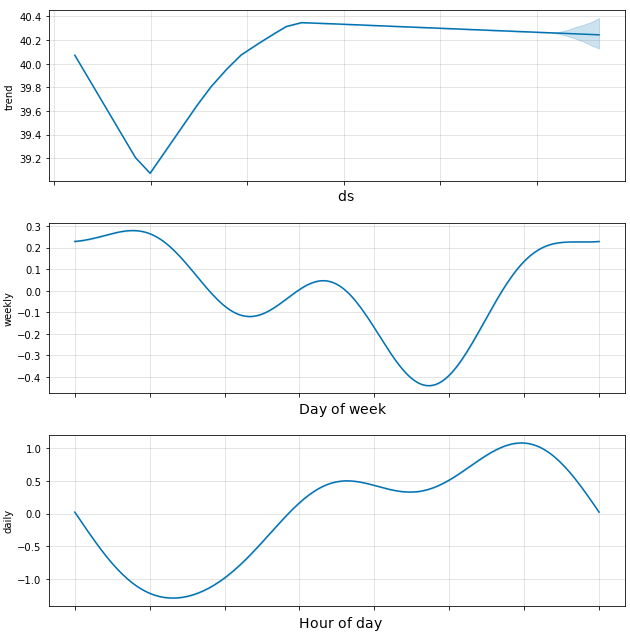
\includegraphics[width=0.65\linewidth]{prophet_uni_components}
	\caption{Learnt components from the univariate Prophet model}
	\label{fig:prophet_uni_components}
\end{figure}

\subsubsection*{Data and predictions joint distribution}

If the joint distributions for the true values $y$ and the predicted values $\hat{y}$ are plotted, it can be seen how the outlier in the training set was not learnt and how the approximation becomes erratic in the test set. Nonetheless, they already show a considerable improvement from the baselines distributions.

\begin{figure}[hptb]
	\centering
	\begin{subfigure}{.49\textwidth}
		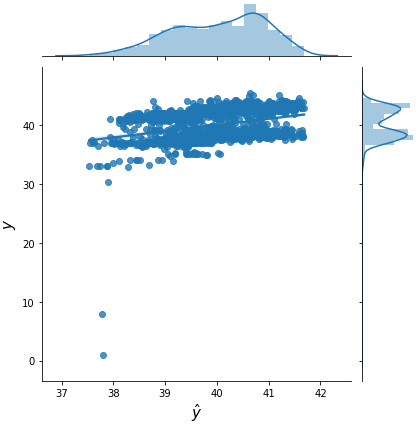
\includegraphics[width=\textwidth]{prophet_train_res_joint}
		\caption{Train}
		\label{fig:prophet_train_res_joint}
	\end{subfigure}%
	\hfill
	\begin{subfigure}{.49\textwidth}
		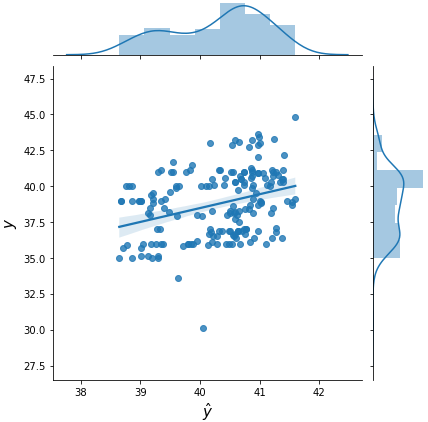
\includegraphics[width=\textwidth]{prophet_test_res_joint}
		\caption{Test}
		\label{fig:prophet_test_res_joint}
	\end{subfigure}
	\caption{Univariate Prophet joint distributions of $y$ and $\hat{y}$}
	\label{fig:prophet_res_joint}
\end{figure}


\subsection{Prophet implementation using exogenous regressors}

To fully exploit the flexibility of \acp{gam}, Prophet's API allows defining custom regressors, which in the current work will be called exogenous variables as a resemblance of SARIMAX models. These variables are the ones explained in Chapter \ref{cha:data_analysis}.

The overall performance can be seen in Figure \ref{fig:prophet_multi_split}. Compared to the univariate model, it can be seen that the confidence bounds now are narrower since there is less uncertainty in the predictions. It also can be seen that the model now can predict the trend change in the test set. 

\begin{figure}[H]
	\centering
	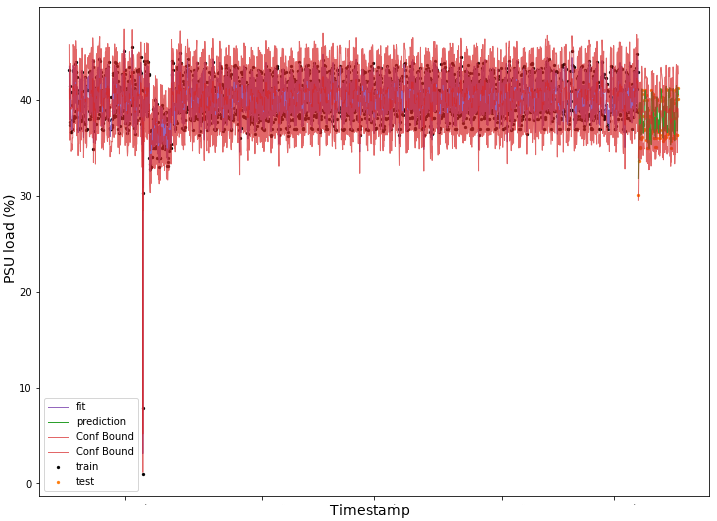
\includegraphics[width=0.8\linewidth]{figures/prophet_multi_split}
	\caption{Training, test and predictions from the multivariate Prophet model}
	\label{fig:prophet_multi_split}
\end{figure}


\subsubsection*{Model learnt components}

The model components now show the additive factor of all the exogenous regressors, which seems to contain the information not learnt by the univariate training residuals. 


%
%The $R^2$ score has considerably improved. Nonetheless, the other scores have become worse. The interpretation of this decline could be that the confidence band is now narrower than the univariate model. Thus, being out of the confidence band is now likely than before.

\begin{figure}[H]
	\centering
	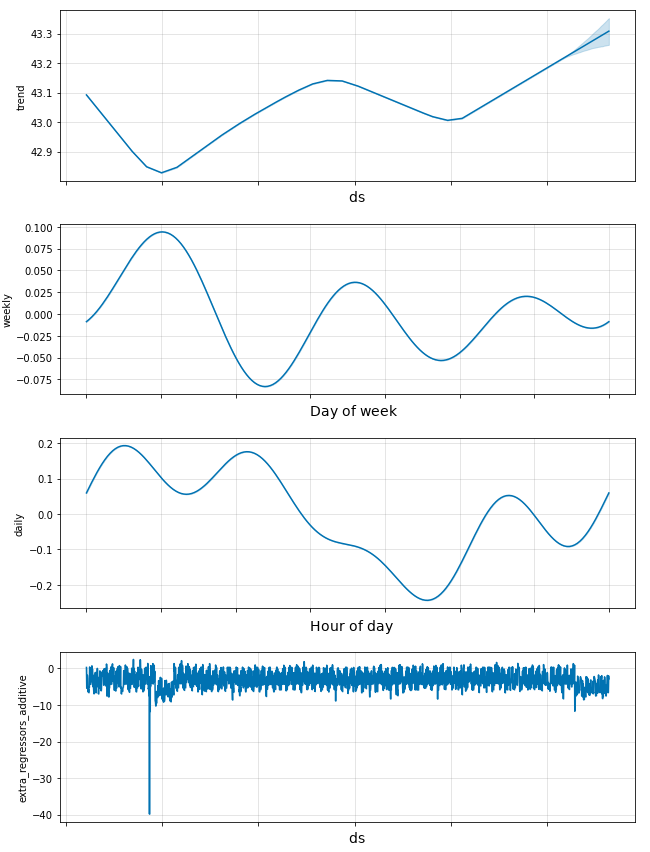
\includegraphics[width=0.65\linewidth]{prophet_multi_components}
	\caption{Learnt components from multivariate Prophet}
	\label{fig:prophet_multi_components}
\end{figure}

\subsubsection*{Data and predictions joint distribution}

The joint distributions for $y$ and $\hat{y}$ in Figure \ref{fig:prophet_test_res_joint_multi} now show that the model has improved significantly  its prediction accuracy compared against the baselines. 

In the plot for the training set, it can be seen that the trend model approximates the abrupt drop. Nonetheless, the positive trend in the correlation between  $y$ and $\hat{y}$ in the test set shows that the model is not overfitting the training data. Moreover, the trend drop in the testing set is also approximated without issues. 

\begin{figure}[hptb]
	\centering
	\begin{subfigure}{.49\textwidth}
		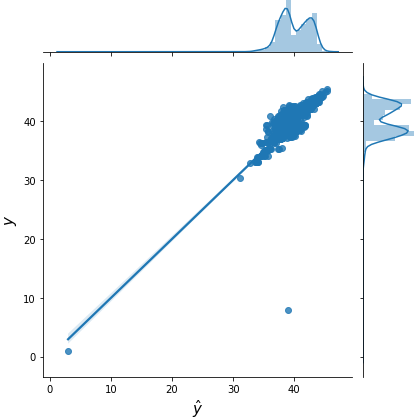
\includegraphics[width=\textwidth]{prophet_train_res_joint_multi}
		\caption{Train}
		\label{fig:prophet_train_res_joint_multi}
	\end{subfigure}%
	\hfill
	\begin{subfigure}{.49\textwidth}
		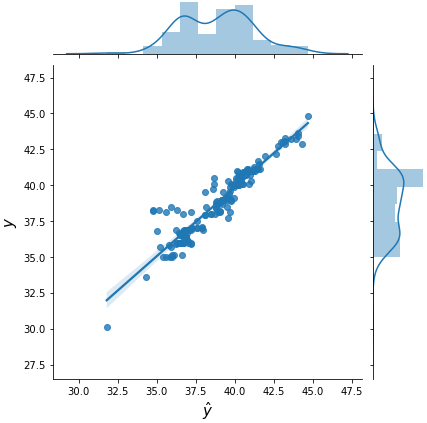
\includegraphics[width=\textwidth]{prophet_test_res_joint_multi}
		\caption{Test}
		\label{fig:prophet_test_res_joint_multi}
	\end{subfigure}
	\caption{Multivariate Prophet joint distributions of $y$ and $\hat{y}$}
	\label{fig:prophet_res_joint_multi}
\end{figure}


\subsection{Example forecast performance comparison}

In order to quantify the improvement of the long-range predictions made by the usage of the Prophet model. Table \ref{table:prophet_scores} summarises the performance scores.

\begin{table}[H]
\centering
\begin{tabular}{|l|c|c|c|c|}
	\hline
					& \ac{mae}	&	$R^2$		& \ac{mobe}  & \ac{rmse} 	\\
	\hline 												
	Univar - Train 	&	2.16	&	0.14		& 	0.04	&	2.53		\\
	Univar - Test 	&	2.11	&	-0.57		&	0.04	&	2.70		\\
	Multivar - Train&	0.55	&	0.83		& 	0.05	&	1.13		\\
	Multivar - Test &	0.57	&\textbf{0.85}	&	0.03	&\textbf{0.85}	\\
	\hline
\end{tabular}
\caption{Example of long-range prediction performance by the Prophet model}
\label{table:prophet_scores}
\end{table}


In this example, the significant improvement done by using the exogenous predictors in the multivariate model can be observed, obtaining a $R^2=0.85$, which for a non-linear case can be considered a good approximation.


\section{Exhaustive forecasting experiments}

After visualising how the models comparatively perform in an example case, a general view of how they perform is needed. Therefore, similar to the experiments in Section \ref{sec:imp-exps}, it is performed an exhaustive iterative evaluation of the predictions is performed while moving the predicting horizon further and further. 

In the following subsections, the exhaustive baseline results are presented, and then Prophet model results are obtained to visualise its general improvement.

\subsection{Baselines predictions moving horizon}

\begin{figure}[htpb]
	\centering
	\begin{subfigure}{.49\textwidth}
		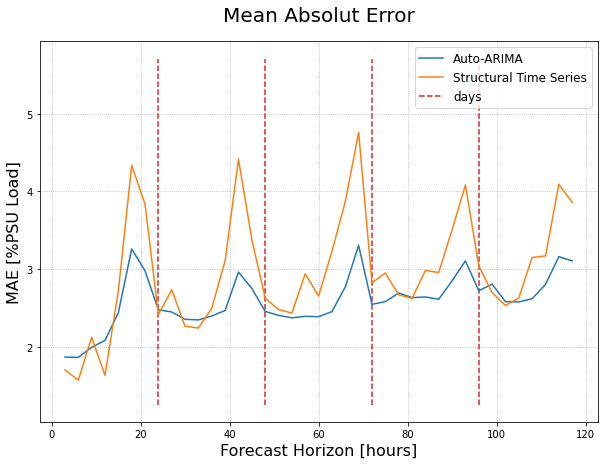
\includegraphics[width=\linewidth]{baseline_db-structts_MAE}
		\caption{Baseline MAE}
	\end{subfigure}%
	\hfill
	\begin{subfigure}{.49\textwidth}
		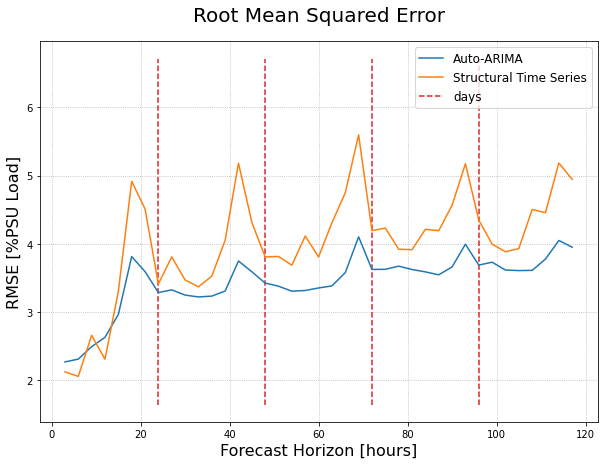
\includegraphics[width=\linewidth]{baseline_db-structts_RMSE}
		\caption{Baseline RMSE}
	\end{subfigure}
	\caption{Baseline predictions performance vs forecast horizon time}
	\label{fig:baseline_performances}
\end{figure}


Figure \ref{fig:baseline_performances} shows the Auto-ARIMA and structural model performances together. The curves are interesting due to their peak-valley seasonal-alike shapes. Their possible explanation is related to the original signal peaks and valleys variability, i.e., the minima are more show less variability than the maxima. Therefore, the predictions for the minima are less error-prone than for the maxima. 

On the other hand, it can be seen that, opposed to the results for the imputation phase, the structural model provides poorer predictions than the ARIMA. Thus, if any of the baselines would have to be chosen, the Auto-ARIMA would be the best candidate.


\subsection{Univariate Prophet prediction moving horizon}
\label{subsec:Results-Experiments-UnivariateProphet}

This set of experiments have been found to require hefty computing power and time. Since the following overall experiment took $\sim17$ hours to finish, it has been limited to sampling 50 models performances for a three days long-range horizon maximum.


%\begin{figure}[H]
%	\centering
%	\begin{subfigure}{0.49\linewidth}
%		\includegraphics[width=\linewidth]{}
%		\caption{}
%	\end{subfigure}
%	\hfill
%	\begin{subfigure}{0.49\linewidth}
%		\includegraphics[width=\linewidth]{}
%		\caption{}
%	\end{subfigure}
%	\caption{}
%	\label{fig:}
%\end{figure}

\begin{figure}[H]
	\centering
	\begin{subfigure}{0.49\linewidth}
		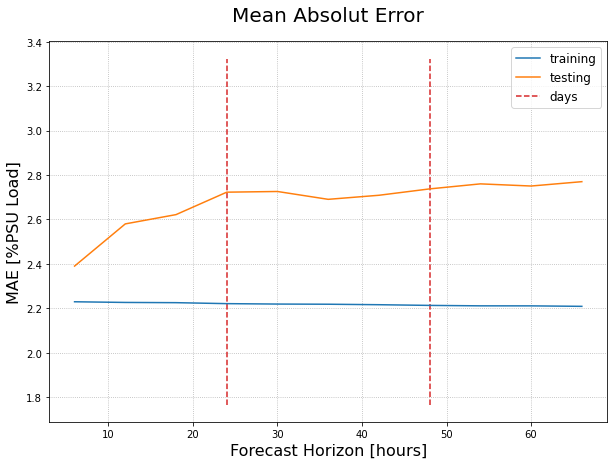
\includegraphics[width=\linewidth]{exp_prophet_uni_mae_time}
		\caption{\ac{mae}}
	\end{subfigure}
	\hfill
	\begin{subfigure}{0.49\linewidth}
		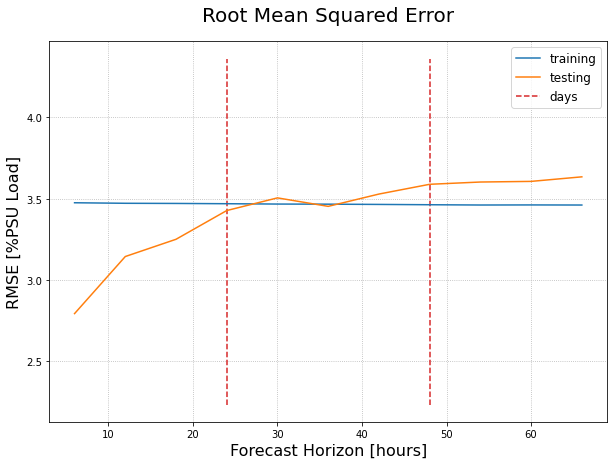
\includegraphics[width=\linewidth]{exp_prophet_uni_rmse_time}
		\caption{\ac{rmse}}
	\end{subfigure}
	\caption{Univariate Prophet predictions performance vs forecast horizon time}
	\label{fig:uni_prophet_performances}
\end{figure}

In the results in Figure \ref{fig:uni_prophet_performances}, it can be observed that as long the time horizon increases, as expected, the prediction errors tend to increase also. While \ac{mae} show that the prediction errors are consistently higher than the training error, the \ac{rmse} shows lower scores for the testing set than for the training when the time horizon is close to the present time. This shift can be explained by the fact that \ac{rmse} penalises higher the large errors compared to \ac{mae}. 

It is important to notice that, as the \ac{psu} utilisation signal is already in percent, these results are easily interpretable as percent error also. Therefore, in the long-range, the univariate Prophet model, shows that in average it can achieve $\text{MAE}\sim2.5$ and $\text{RMSE} \sim 3.6$ \ac{psu} per-cent utilisation.

%\subsubsection*{Mean Absolut Error}
%\begin{figure}[H]
%	\centering
%	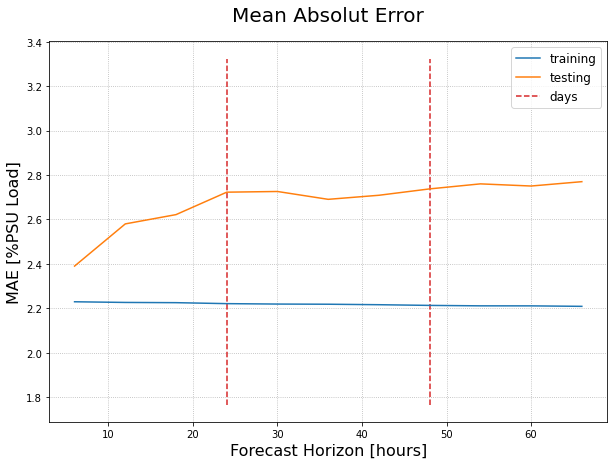
\includegraphics[width=0.8\linewidth]{exp_prophet_uni_mae_time}
%	\caption{Univariate moving prediction horizon: \ac{mae}}
%	\label{fig:exp_prophet_uni_mae}
%\end{figure}
%
%\subsubsection*{Root Mean Squared Error}
%\begin{figure}[H]
%	\centering
%	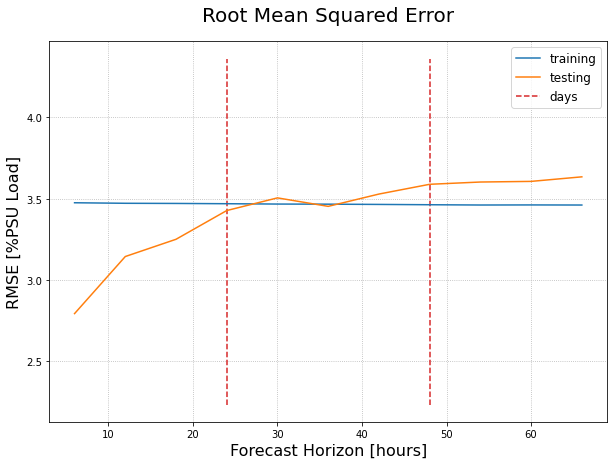
\includegraphics[width=0.8\linewidth]{exp_prophet_uni_rmse_time}
%	\caption{Univariate moving prediction horizon: \ac{rmse}}
%	\label{fig:exp_prophet_uni_rmse}
%\end{figure}



\subsection{Multivariate Prophet prediction moving horizon}

Now it is the turn of the Prophet model with external regressors that showed the best performance in the first example. Therefore, it is expected to maintain that tendency but now with more confidence that the performance in the example was not some fortunate random event.

These experiments have consumed even more computing time than the previous in Section \ref{subsec:Results-Experiments-UnivariateProphet}, having spent more than 18.5 hours to finish.

\begin{figure}[H]
	\centering
	\begin{subfigure}{0.49\linewidth}
		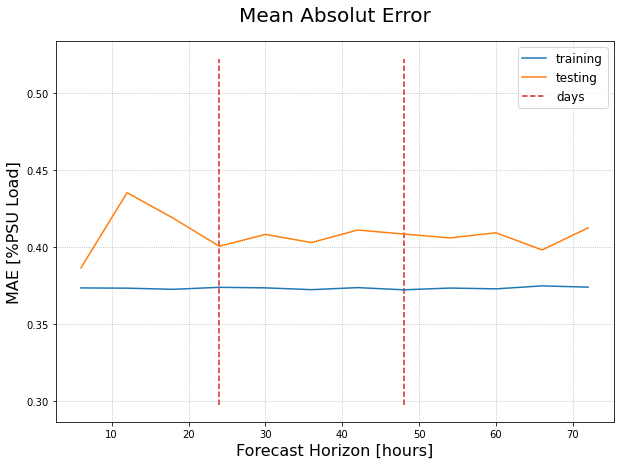
\includegraphics[width=\linewidth]{exp_prophet_mv_mae_time}
		\caption{\ac{mae}}
	\end{subfigure}
	\hfill
	\begin{subfigure}{0.49\linewidth}
		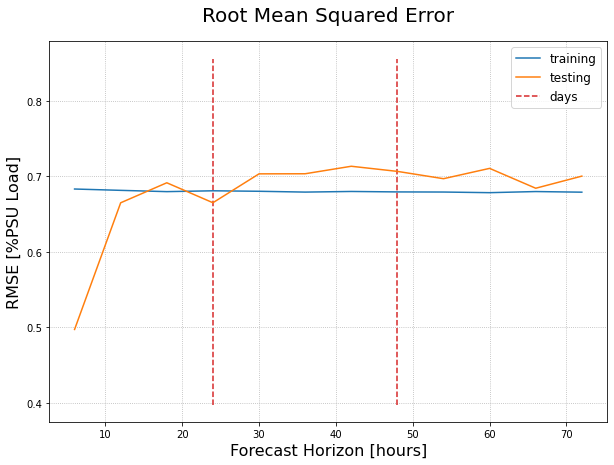
\includegraphics[width=\linewidth]{exp_prophet_mv_rmse_time}
		\caption{\ac{rmse}}
	\end{subfigure}
	\caption{Multivariate Prophet predictions performance vs forecast horizon time}
	\label{fig:multi_prophet_performances}
\end{figure}

The results in Figure \ref{fig:multi_prophet_performances} show that the long-range prediction results for the Prophet model using exogenous regressors are consistently good having both, $\text{MAE}$ and $\text{RMSE}$ below $1\%$.

%\begin{figure}[H]
%	\centering
%	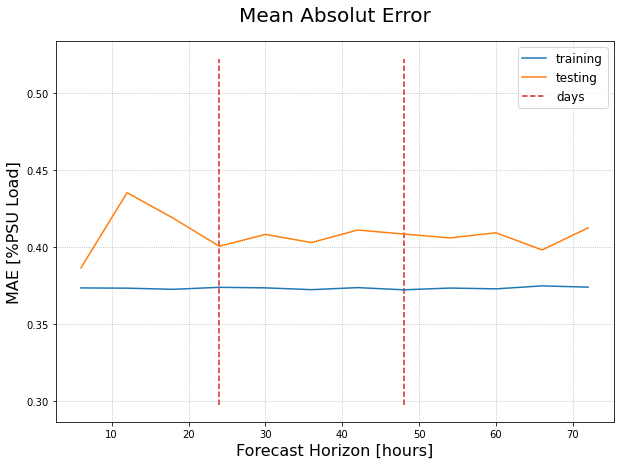
\includegraphics[width=0.8\linewidth]{exp_prophet_mv_mae_time}
%	\caption{Multivariate moving prediction horizon: \ac{mae}}
%	\label{fig:exp_prophet_mv_mae}
%\end{figure}
%\begin{figure}[H]
%	\centering
%	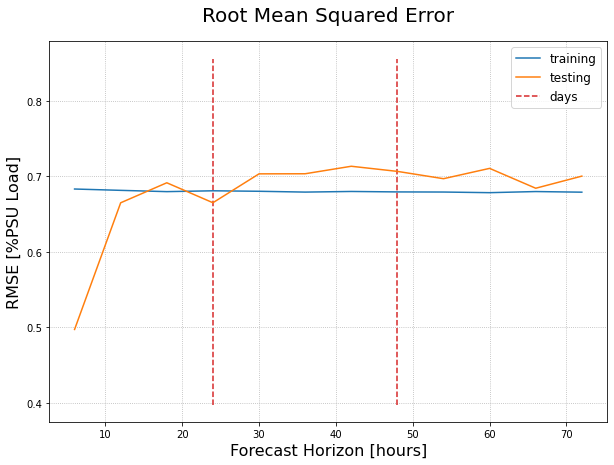
\includegraphics[width=0.8\linewidth]{exp_prophet_mv_rmse_time}
%	\caption{Multivariate moving prediction horizon: \ac{rmse}}
%	\label{fig:exp_prophet_mv_rmse}
%\end{figure}

Other noticeable results are the ones shown in Figure \ref{fig:exp_prophet_mv_r2}, in which the $R^2$ scores in long-range are $\sim0.88$. Although it might seem unintuitive to have better $R^2$ in the long-range rather than in the short term, it can be explained by the amount of data used to compute the score: the less data, the more likely to have \emph{a general bad approximation}. 

\begin{figure}[H]
	\centering
	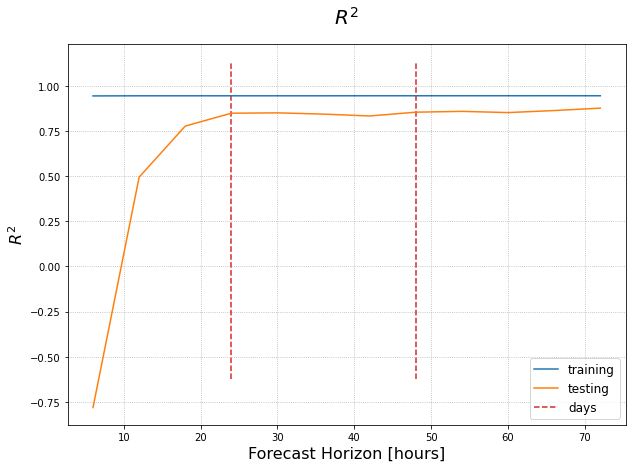
\includegraphics[width=0.65\linewidth]{exp_prophet_mv_r2_time}
	\caption{Multivariate Prophet model $R^2$ vs forecast horizon time}
	\label{fig:exp_prophet_mv_r2}
\end{figure}

\subsection{Time performances}

Figure \ref{fig:time-perfs} shows the average consumed time for running the exhaustive experiments in Ericsson's computing farm. It can be seen that the testing time is very similar for univariate and multivariate case. On the other hand, the training time for the multivariate model is slightly higher than the univariate one. Nonetheless, both are under half of a second on average. It is also interesting that the longer the prediction range, the times remain almost constant.

\begin{figure}[H]
	\centering
	\begin{subfigure}{0.49\linewidth}
		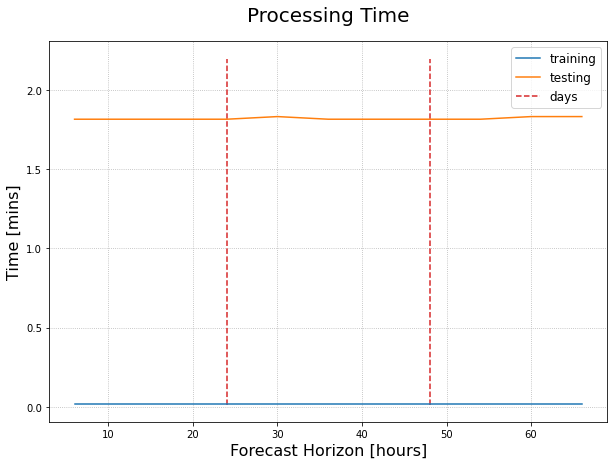
\includegraphics[width=\linewidth]{exp_prophet_uni_time}
		\caption{Univariate experiment computing time}
	\end{subfigure}
	\hfill
	\begin{subfigure}{0.49\linewidth}
		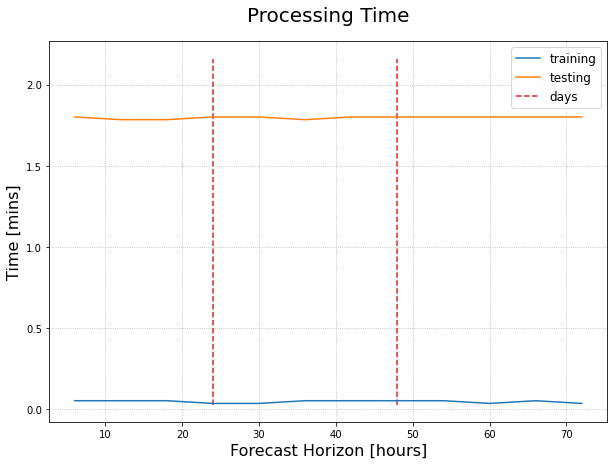
\includegraphics[width=\linewidth]{exp_prophet_mv_time}
		\caption{Multivariate experiment computing time}
	\end{subfigure}
	\caption{Experiments computing times}
	\label{fig:time-perfs}
\end{figure}



\section{Performance summary}

Finally, for ease of comparison this section summarises the average performances per day for all the models under analysis. Table \ref{table:mae_perf_summary} shows that the Prophet model with exogenous regressors vastly outperforms the other methods in terms of \ac{mae}.

\begin{table}[H]
	\centering
	\begin{tabular}{|c|c|c|c|}
		\hline
		\textbf{Model} & \textbf{1 day} & \textbf{2 day}	& \textbf{3 day} \\
		\hline
		Structural		 & 		2.55 	&		3.17 		& 3.08 			\\
		\hline
		ARIMA 			 &		2.59 	& 		2.812		& 2.70 			\\
		\hline
		UniVar-Prophet 	 & 		2.88 	& 		2.96 		& 3.01 			\\
		\hline
		MultiVar-Prophet & \textbf{0.41}& \textbf{0.40}		& \textbf{0.40} \\
		\hline
	\end{tabular}
	\caption{\ac{mae} Summary of models performance by day}
	\label{table:mae_perf_summary}
\end{table}

Likewise, in Table \ref{table:rmse_perf_summary}, it can be observed the long-range stability of the multivariate Prophet model having, again, the best \ac{rmse} scores.

\begin{table}[H]
	\centering
	\begin{tabular}{|c|c|c|c|}
		\hline
		\textbf{Model} & \textbf{1 day} & \textbf{2 day}	& \textbf{3 day} \\
		\hline
		Structural		 & 		3.27 	&		4.31 		& 4.35 			\\
		\hline
		ARIMA 			 &		3.22 	& 		3.77		& 3.81 			\\
		\hline
		UniVar-Prophet 	 & 		3.54	& 		3.88		& 4.02 			\\
		\hline
		MultiVar-Prophet & \textbf{0.62}& \textbf{0.71} 	& \textbf{0.68}	\\
		\hline
	\end{tabular}
	\caption{\ac{rmse} Summary of models performance by day}
	\label{table:rmse_perf_summary}
\end{table}

Lastly, Table \ref{table:r2_perf_summary} presents how the multivariate Prophet model is even capable of having acceptable $R^2$ scores, which in this type of data is not an easy task.

\begin{table}[H]
	\centering
	\begin{tabular}{|c|c|c|c|}
		\hline
		\textbf{Model} & \textbf{1 day} & \textbf{2 day}	& \textbf{3 day} \\
		\hline
		Structural		 & 		-7.23 	&		-8.90 		& -2.90 		  \\
		\hline
		ARIMA 			 &		-95.76 	& 		-2.25		& -0.23 		  \\
		\hline
		UniVar-Prophet 	 & 		-203.76	& 		-1.04 		& -0.98 	      \\
		\hline
		MultiVar-Prophet & \textbf{0.33}& 	\textbf{0.85} 	& \textbf{0.86} \\
		\hline
	\end{tabular}
	\caption{$R^2$ Summary of models performance by day}
	\label{table:r2_perf_summary}
\end{table}



\section{Power headroom estimation}

Until this point of the work, the research has been mainly focused on PSU loads forecasting. Nonetheless, as mentioned in the introductory context, the goal is to predict the power headroom defined in (\ref{eq:phdroom}). However, as there are no direct measurements of power headroom that can be learnt, it needs to be derived from the power consumption.  

Therefore, to provide a power headroom forecast, after estimating the loads future values, a further step is needed to translate that information into power headroom terms. The following sections will propose a way to manage to achieve it and discuss other aspects of its technical applicability.

\subsection{Power headroom derivation as PSU utilisation complement}

As it has been exposed in Section \ref{subsec:data_description:power_supply}, the power load is a measure of \emph{how many percentual power capacity it is being used at that time}. Thus, it is straightforward to claim that the percentual power headroom is its complement.

\begin{align}\label{eq:ph_deriv}
	\begin{split}
		P_{h[\%]}	&= 100 - P_{L[\%]} \\
		\text{Where }P_{h[\%]}	&: \text{Power headroom in percents} \\
		\text{and } P_{L[\%]}	&: \text{Power loads consumptions in percents}
	\end{split}
\end{align}

If the interest is to obtain a measurement in Watts units, the installed power capacity in the RBS, $P_{max}$, needs to be known so that its proportion can be computed as showed in (\ref{eq:phwatts}).

\begin{align}\label{eq:phwatts}
	\begin{split}
		P_h	&= P_{max} \cdot \frac{P_{h[\%]}}{100} \\
		\text{Where } P_{max}	&: \text{Installed power capacity in Watts}
	\end{split}
\end{align}

Figure \ref{fig:ph_der}, shows the \ac{psu} utilisation signal used as example test in Chapter \ref{cha:forecasting} and its derived power headroom.
 	

%\begin{figure}[H]
%	\centering
%	\begin{subfigure}{0.49\linewidth}
%		\includegraphics[width=\linewidth]{}
%		\caption{}
%	\end{subfigure}
%	\hfill
%	\begin{subfigure}{0.49\linewidth}
%		\includegraphics[width=\linewidth]{}
%		\caption{}
%	\end{subfigure}
%	\caption{}
%	\label{fig:}
%\end{figure}

\begin{figure}[H]
	\centering
	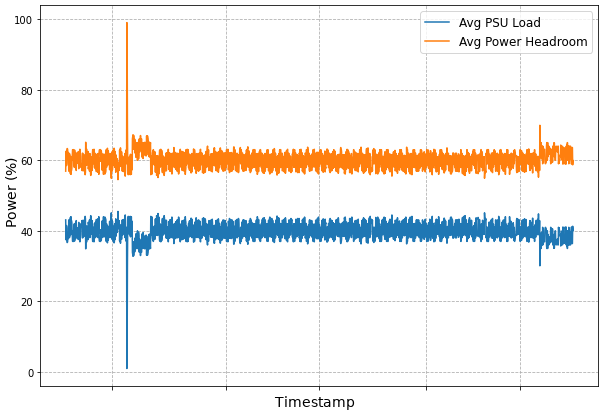
\includegraphics[width=0.65\linewidth]{power_headroom_derivation}
	\caption{Power headroom derivation from PSU Load}
	\label{fig:ph_der}
\end{figure}


%\begin{figure}[hptb]
%	\centering
%	\begin{subfigure}{.65\textwidth}
%		\centering
%		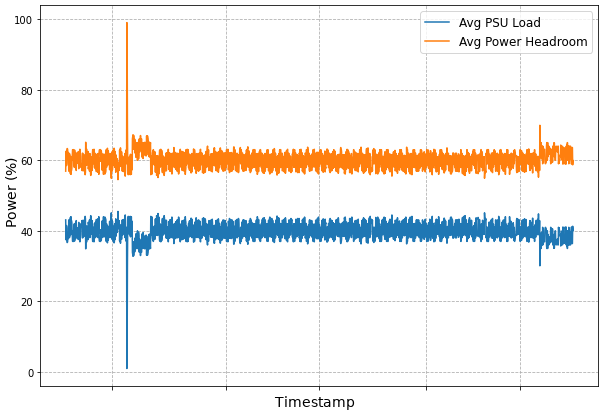
\includegraphics[width=\textwidth]{power_headroom_derivation}
%		\caption{Derived power headroom in percents}
%		\label{fig:ph_der_percent}
%	\end{subfigure}%
%	\hfill
%	\begin{subfigure}{.65\textwidth}
%		\centering
%		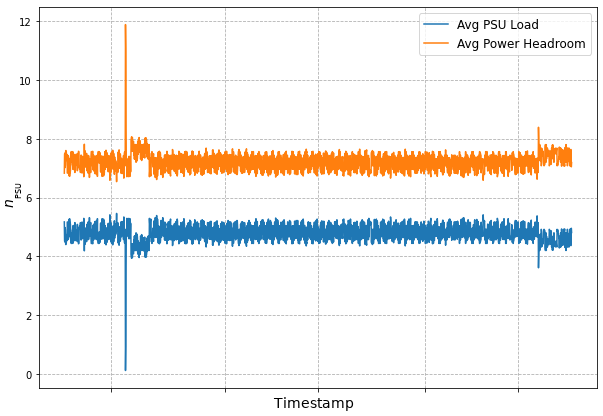
\includegraphics[width=\textwidth]{power_headroom_derivation_watts}
%		\caption{Derived power headroom in Watts}
%		\label{fig:ph_der_watts}
%	\end{subfigure}
%	\caption{Power headroom derivation from PSU Load}
%	\label{fig:ph_der}
%\end{figure}

\subsection{Criterion considerations}

In general terms, an alarm is meant to make someone notice that something abnormal is happening in a given process or, in a forecasting context, may (or will) occur in the future, to support the operator response \cite{iec_alarms}.

In the present works' context, the alarm meaning can be conceived as the \ac{rbs} not having enough power to maintain its by-design behaviour.

Although it should be possible to define how likely a power overload is, given the system's current state in probability terms, triggering an alarm is a binary task. The system is operating either in a \emph{"safe"}  or in an \emph{"abnormal"} region. Then, crossing a boundary that separates these two regions is the trigger for the alarm. 

There are different techniques to tune an optimal trigger level. It could be done based on a system variable, or latent variable, or even a joint distribution of the two kinds \cite{izadi2009alarms}. 

Choosing the best possible boundary is considered to be out of scope. Nonetheless, as an initial approach, it can be proposed to be settable by the user according to their needs and expertise. 

From this assumption and the derivations in (\ref{eq:ph_deriv}) and (\ref{eq:phwatts}), the following guidelines should be taken into consideration. 

\subsubsection*{Values interpretation}

Percentages values are not always able to fully represent the system conditions. For example, it is very different having 10\% of power headroom where the total capacity is 10 kW and 1 kW since the relative oscillations could be drastically different. Therefore, the power magnitude should be taken into consideration. 

\subsubsection*{PSUs do not partially fail}

The power capacity is not continuous. It will have discrete values as shown in Figure \ref{fig:ph_lvls}, and also, the \acp{psu} can have different power contributions. This quantisation means that in order to set the threshold is needed to take into account the worst-case scenario, which can be depicted by the sentence: \emph{"can the \ac{rbs} work if the next failure is the most power contributing \ac{psu}?"}

%\begin{figure}[hptb]
%	\centering
%	\begin{subfigure}{.65\textwidth}
%		\centering
%		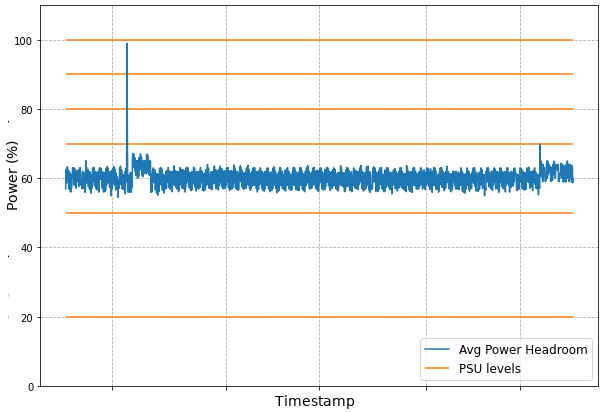
\includegraphics[width=\textwidth]{power_headroom_levels_percent}
%		\caption{Power headroom and discrete availability in percents}
%		\label{fig:ph_lvls_percent}
%	\end{subfigure}%
%	\hfill
%	\begin{subfigure}{.65\textwidth}
%		\centering
%		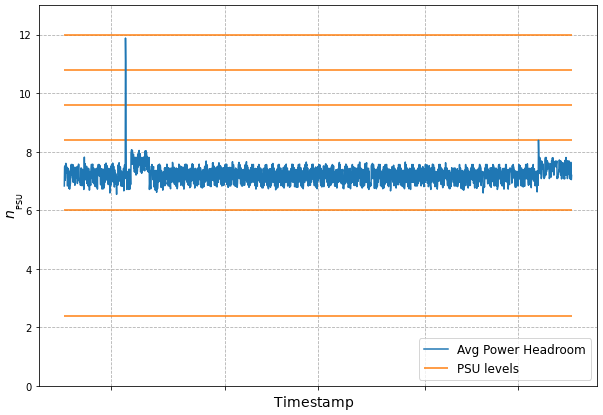
\includegraphics[width=\textwidth]{power_headroom_levels_watts}
%		\caption{Power headroom and discrete availability in Watts}
%		\label{fig:ph_lvls_watts}
%	\end{subfigure}
%	\caption{Power headroom derivation from PSU Load}
%	\label{fig:ph_lvls}
%\end{figure}

\begin{figure}[hptb]
	\centering
	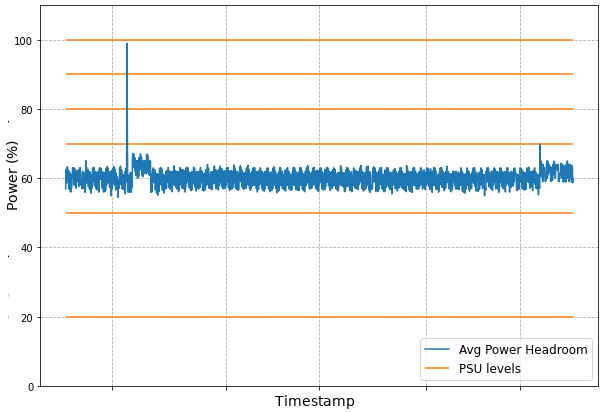
\includegraphics[width=.65\textwidth]{power_headroom_levels_percent}
	\caption{Power headroom and discrete availability in percents}
	\label{fig:ph_lvls}
\end{figure}

\pagebreak
\subsection{Alarm triggering and the $n$-level safety criteria}

Let $P_{max}$ be the maximum power capacity installed and working in an \ac{rbs},  $\bar{P}_{Load}$ the average \ac{psu} utilisation and $\Delta p$ the confidence interval used when training the Prophet model. Let $N$ be the amount of working \acp{psu}, let $\{P_{PSU_1}, \ldots, P_{PSU_N}\}$ such that $P_{PSU_1} > \ldots > P_{PSU_N}$ are the descending sorted power contributions from the working \acp{psu}.

Then, let the $n$-level safety criteria, be the $n$ amount of worst-case \ac{psu} failures to keep as operational margin:

\begin{align}
	\begin{split}
		P_{max} - \sum_{i=1}^{n}{P_{PSU_i}} &> \bar{P}_{Load} + \Delta p \\
		P_{max} - \left\{\bar{P}_{Load} + \Delta p \right\} &> \sum_{i=1}^{n}{P_{PSU_i}}
	\end{split}
\end{align}

However, as the power headroom is by definition the difference between the installed power capacity and the power being consumed, it can be said that: 

\begin{align}
	\begin{split}
		P_{h} &= P_{max} - \left\{\bar{P}_{Load} + \Delta p \right\} \\
		P_{h} &> \sum_{i=1}^{n}{P_{PSU_i}} \\
		\therefore P_{crit_n} &= \sum_{i=1}^{n}{P_{PSU_i}}
	\end{split}
\end{align} 

Where $ P_{crit_n}$ is the $n$-level criteria threshold. Thus, whenever the power headroom forecast $\hat{P}_h$ at time $t+k$, $t$ being the current time, meets the condition in (\ref{eq:n-trigger}) a fault alarm must be triggered

\begin{equation}
	\label{eq:n-trigger}
	\hat{P}_{h_{t+k}} \geq P_{crit_n}
\end{equation}







